\PassOptionsToPackage{unicode=true}{hyperref} % options for packages loaded elsewhere
\PassOptionsToPackage{hyphens}{url}
%
\documentclass[12pt,english,]{article}
\usepackage{lmodern}
\usepackage{amssymb,amsmath}
\usepackage{ifxetex,ifluatex}
\usepackage{fixltx2e} % provides \textsubscript
\ifnum 0\ifxetex 1\fi\ifluatex 1\fi=0 % if pdftex
  \usepackage[T1]{fontenc}
  \usepackage[utf8]{inputenc}
  \usepackage{textcomp} % provides euro and other symbols
\else % if luatex or xelatex
  \usepackage{unicode-math}
  \defaultfontfeatures{Ligatures=TeX,Scale=MatchLowercase}
\fi
% use upquote if available, for straight quotes in verbatim environments
\IfFileExists{upquote.sty}{\usepackage{upquote}}{}
% use microtype if available
\IfFileExists{microtype.sty}{%
\usepackage[]{microtype}
\UseMicrotypeSet[protrusion]{basicmath} % disable protrusion for tt fonts
}{}
\usepackage{hyperref}
\hypersetup{
            pdfauthor={Minh Thang Cao},
            pdfborder={0 0 0},
            breaklinks=true}
\urlstyle{same}  % don't use monospace font for urls
\usepackage[margin=1in]{geometry}
\usepackage{graphicx,grffile}
\makeatletter
\def\maxwidth{\ifdim\Gin@nat@width>\linewidth\linewidth\else\Gin@nat@width\fi}
\def\maxheight{\ifdim\Gin@nat@height>\textheight\textheight\else\Gin@nat@height\fi}
\makeatother
% Scale images if necessary, so that they will not overflow the page
% margins by default, and it is still possible to overwrite the defaults
% using explicit options in \includegraphics[width, height, ...]{}
\setkeys{Gin}{width=\maxwidth,height=\maxheight,keepaspectratio}
\setlength{\emergencystretch}{3em}  % prevent overfull lines
\providecommand{\tightlist}{%
  \setlength{\itemsep}{0pt}\setlength{\parskip}{0pt}}
\setcounter{secnumdepth}{0}
% Redefines (sub)paragraphs to behave more like sections
\ifx\paragraph\undefined\else
\let\oldparagraph\paragraph
\renewcommand{\paragraph}[1]{\oldparagraph{#1}\mbox{}}
\fi
\ifx\subparagraph\undefined\else
\let\oldsubparagraph\subparagraph
\renewcommand{\subparagraph}[1]{\oldsubparagraph{#1}\mbox{}}
\fi

% set default figure placement to htbp
\makeatletter
\def\fps@figure{htbp}
\makeatother

\usepackage{float}
\usepackage[boxruled,vlined]{algorithm2e}
\usepackage{listings}
\usepackage{xcolor}
\usepackage {tikz}
\usepackage{indentfirst}
\usepackage{tabularx}
\usepackage{multirow}
\usepackage{pgfplots}
\usepackage[bottom]{footmisc}
% \definecolor{listinggray}{gray}{0.9}
% \definecolor{lbcolor}{rgb}{0.9,0.9,0.9}
% \definecolor{Darkgreen}{rgb}{0,0.4,0}
% \lstset{
% backgroundcolor=\color{lbcolor},
%     tabsize=2,    
%   rulecolor=,
%     language=[GNU]C++,
%     basicstyle=\scriptsize,
%     upquote=true,
%     aboveskip={1.5\baselineskip},
%     columns=fixed,
%     showstringspaces=false,
%     extendedchars=false,
%     breaklines=true,
%     prebreak = \raisebox{0ex}[0ex][0ex]{\ensuremath{\hookleftarrow}},
%     frame=single,
%     numbers=left,
%     showtabs=false,
%     showspaces=false,
%     showstringspaces=false,
%     identifierstyle=\texttt,
%     keywordstyle=\color[rgb]{0,0,1},
%     commentstyle=\color[rgb]{0.026,0.112,0.095},
%     stringstyle=\color[rgb]{0.627,0.126,0.941},
%     numberstyle=\color[rgb]{0.205, 0.142, 0.73},
% }
% 
% \lstset{
%   backgroundcolor=\color{lbcolor},
%   tabsize=2,
%   language=C++,
%   captionpos=b,
%   tabsize=3,
%   frame=lines,
%   numbers=left,
%   numberstyle=\tiny,
%   numbersep=5pt,
%   breaklines=true,
%   showstringspaces=false,
%   basicstyle=\footnotesize,
%  identifierstyle=\color{magenta},
%   keywordstyle=\color[rgb]{0,0,1},
%   commentstyle=\color{Darkgreen},
%   stringstyle=\color{red}
%   }
\colorlet{mygray}{black!30}
\colorlet{mygreen}{green!60!black}
\colorlet{mymauve}{red!90}

\lstset{
  tabsize=2,
  backgroundcolor=\color{gray!10},  
  basicstyle=\ttfamily,
  columns=fullflexible,
  breakatwhitespace=false,      
  breaklines=true,                
  captionpos=b,                    
  commentstyle=\color{mygreen}, 
  extendedchars=true,              
  frame=single,                   
  keepspaces=true,             
  keywordstyle=\bfseries\color{blue},      
  language=c++,                 
  numbers=left,                
  numbersep=5pt,
  breaklines=true,
  numberstyle=\tiny, 
  rulecolor=\color{mygray},        
  showspaces=false,               
  showtabs=true,                                  
  stringstyle=\color{mymauve},                          
  title=\lstname                
}

\definecolor{light-gray}{gray}{0.9}
\newcommand{\code}[1]{\colorbox{light-gray}{\texttt{#1}}}
\newcommand{\pnt}[1]{{\scriptstyle#1}}
\let\origfigure\figure
\let\endorigfigure\endfigure
\renewenvironment{figure}[1][2] {
    \expandafter\origfigure\expandafter[H]
} {
    \endorigfigure
}
\usepackage{etoolbox}
\makeatletter
\providecommand{\subtitle}[1]{% add subtitle to \maketitle
  \apptocmd{\@title}{\par {\large #1 \par}}{}{}
}
\makeatother
\ifnum 0\ifxetex 1\fi\ifluatex 1\fi=0 % if pdftex
  \usepackage[shorthands=off,main=english]{babel}
\else
  % load polyglossia as late as possible as it *could* call bidi if RTL lang (e.g. Hebrew or Arabic)
  \usepackage{polyglossia}
  \setmainlanguage[]{english}
\fi

\title{\textbf{Project Report}\\
\Large{An Implementation Of:}}
\providecommand{\subtitle}[1]{}
\subtitle{A Simple Randomized \(O(n\,\log\, n)\)--Time Closest-Pair\\
Algorithm in Doubling Metrics}
\author{Minh Thang Cao}
\date{31 July 2020}

\begin{document}
\maketitle

\hypertarget{section1}{%
\section{\texorpdfstring{1
\enspace Introduction}{1 Introduction}}\label{section1}}

Implementation of an algorithm helps us observe its efficiency and
behavior in practice. In this report, I will briefly explain each part
of the closest-pair doubling algorithm {[}1{]}, show the program's
implementation along with practical running time analysis, and some
implementation techniques I used. The theoretical information in this
report fully refers to the work of A. Maheshwari, W. Mulzer and M. Smid,
see {[}1{]}.

Given a metric space \((P,dist)\), with doubling dimension \(d\), whose
\(P\) is a set of \(n\) points. The closest pair of points is the two
points with the distance \(\delta_0\) that satisfies
\(dist(p_1, p_2) \geq \delta_0\) for any point \(p_1, p_2 \in P\). Also,
the doubling dimension \(d\) of a metric space indicates that for every
point \(p\) in \(P\) and every real number \(R > 0\), the
\(ball_P(p, R)\) can be covered by at most \(2^d\) balls in \(P\) of
radius \(R/2\), see {[}1, Section 2{]}. By using the definition and
properties of the doubling metric space and its doubling dimension, the
algorithm will find the closest-pair distance without the direct use of
the points' coordinates in \(O(n\,log\,n)\) time.

The closest-pair algorithm consists of three smaller parts:

\vspace{-2.5truemm}

\begin{quote}
\begin{enumerate}
\item Computing a separating annulus, denoted \textsc{SepAnn}$(S,n,d,\mu,c)$
\item The refinement of \textsc{SepAnn}$(S,n,d,\mu,c)$, denoted \textsc{SparseSepAnn}$(S,n,d,t)$
\item The main recursive closest-pair algorithm, denoted \textsc{ClosestPair}$(S,n,d)$
\end{enumerate}
\end{quote}

\vspace{-2truemm}

Throughout the paper, let:

\vspace{-2truemm}

\begin{quote}
\begin{itemize}
\item $(P, dist)$ be a finite metric space in which $P$ is the set of all points, and $dist$ is the function that calculate the distance between any two points
\item $d$ be the space's doubling dimension
\item $S$ be a non-empty subset of $P$
\end{itemize}
\end{quote}

\vspace{-2truemm}

\underline{\emph{\textbf{Note}}}: I will only mention 2D points because
of the extremely high running time of the algorithm in the space more
than 3D (in which the doubling dimension is approximately at least
\(\log_2 21\) that gives us the base case with more than \(3\,000\,000\)
points). \unboldmath

\newpage

\hypertarget{section2}{%
\section{\texorpdfstring{2 \enspace Algorithm 1: Computing a separating
annulus}{2 Algorithm 1: Computing a separating annulus}}\label{section2}}

An important part of the main closest-pair algorithm is finding a
separating annulus in the subset \(S\). I will briefly describe this
algorithm in the next subsection, due to A. Maheshwari, W. Mulzer and M.
Smid {[}1, Section 3.1{]}.

\hypertarget{section2.1}{%
\subsection{\texorpdfstring{2.1 The
\(\mathrm{S\pnt{EP}A\pnt{NN}}(S,n,d,\mu,c)\)
algorithm}{2.1 The \textbackslash{}mathrm\{S\textbackslash{}pnt\{EP\}A\textbackslash{}pnt\{NN\}\}(S,n,d,\textbackslash{}mu,c) algorithm}}\label{section2.1}}

In this section, \(\mu \ge1\) is a real constant number, \(c\) is
calculated based on \(\mu\) (I would say that \(c = 2(4\mu)^d\) {[}1,
Remark 1{]} since \(\mu\) is not an integer in this case {[}1, Section
3.2{]}).

This algorithm picks a uniformly random point \(p\) from the subset
\(S\) then finds the smallest ball centered at \(p\), denoted
\(ball_S(p, R_p)\), that contains at least \(n/c\) point. If the outer
ball \(ball_S(p,\mu R_p)\) contains at most \(n/2\) points, it returns
\(p\) and \(R_p\). If not, this procedure is repeated until the
condition is satisfied. This algorithm's pseudocode is given below, see
{[}1, Section 3.1{]}.

\begin{figure}[ht]
  \centering
  \begin{minipage}{0.9\linewidth}
    {\LinesNotNumbered
    \begin{algorithm}[H]
    \SetKwInOut{Input}{Input}
    \Input{Let $S$ be a subset of $P$, of size $n$, $d$ be the metric space's doubling dimension, $\mu \geq 1$ and $c >1$ be large enough real numbers. }

    \SetKwInOut{Output}{Output}
    \Output{A point $p \in S$ and a radius $R_p > 0$.}
    \DontPrintSemicolon
    \SetAlgoLined
    \BlankLine

    \centering
    \begin{minipage}{.80\linewidth}
    \Repeat{$|ball_S(p, \mu R_p)| \leq n/2$}
      {p = a uniformly random point in $S$;

      $R_p$ = min\{$r > 0: |ball_S(p, r)| \geq n/c$\};}
      return $p$ and $R_p$
    \end{minipage}
    \caption{\textsc{SparseSepAnn}$(S,n,d,t)$}
    \end{algorithm}}
  \end{minipage}
  \begin{minipage}{0.90\textwidth}
    \begin{flushright}
    {\footnotesize \emph{This pseudocode is from [1, Section 3.1]}\par}
    \end{flushright}
  \end{minipage}
\end{figure}

\hypertarget{section2.2}{%
\subsection{\texorpdfstring{2.2 \enspace Finding the \(K^{th}\) smallest
element}{2.2 Finding the K\^{}\{th\} smallest element}}\label{section2.2}}

One step in \textsc{SepAnn($S,n,d,\mu,c$)} algorithm is to find the
smallest ball which contains at least \(n/c\) points. This ball is easy
to find using the \(k^{th}\) smallest element algorithm. Particularly,
in a list of distances between \(p\) and all other points in \(S\), we
pick the \(\lceil n/c\rceil\)-th smallest element and let it be the
radius of the ball we need to find. Thus, all points closer to \(p\) are
inside this ball.

A very easy approach to find the \(k^{th}\) smallest element in a list
is to sort it in ascending order, and then simply return the element at
the \(k^{th}\) place. This sorting algorithm takes \(O(n\,\log\,n)\)
time complexity in the worst case. Fortunately, we can improve the
running time to \(O(n)\) using a common recursive technique called
QuickSelect, which is similar to QuickSort.

Given an unordered list \(D\) which contains \(n\) numbers, and a
positive integer \(k\) satisfies \(1 \leq k \leq n\). Each element in
\(D\) has an index from \(0\) to \(n-1\). Consider a sublist of \(D\),
denoted \(D[a:b]\), which starts from index \(a\) and ends at \(b\),
inclusively. The base case is when \(a = b\), the algorithm returns the
only element in that sublist. If it is not the case, the algorithm will
choose a random \emph{pivot} in the list. The algorithm then rearranges
the list so that all elements smaller and larger than the pivot are to
the left and right of it, respectively. Now, the pivot has a new index,
says \(c\). If \(k = c-a+1\), the chosen pivot is the \(k^{th}\)
smallest element of \(D\), the algorithm returns \(D[c]\). If
\(k < c-a+1\), the algorithm recurses on the sublist to the left of the
pivot, \(D[a:c-1]\). If \(k > c-a+1\), the algorithm recurses on the
sublist to the right of the pivot, \(D[c+1:b]\), with a different input
\(k\) (which is \(k - c + a -1\)) since this is the \(k\) of the subset
to the right, not the whole set of points, and the elements' indices
starts from 0 again when we recurse. This algorithm's pseudocode is
given below.

\begin{figure}[ht]
  \centering
  \begin{minipage}{.9\linewidth}
    {\LinesNotNumbered
    \SetAlgoRefName{}
    \begin{algorithm}[H]
    \SetKwInOut{Input}{Input}
    \Input{Let $D$ be a list of double numbers, the integers $a$ and $b$ respectively be the starting and ending indices of a sublist and $k$ be an integer refers to the $k^{th}$ smallest element.}
    \SetKwInOut{Output}{Output}
    \Output{The $k^{th}$ smallest element in $D$, a double number.}
    \SetAlgoLined
    \BlankLine
    \centering
    \begin{minipage}{.75\linewidth}
        \uIf{$a == b$} {
            return $D[i]$
        }\Else {
      $p$ = a random element in $D$;
      
      \SetKwBlock{partitioning}{\textnormal{\textbf{rearranging:}}}{end;}

      \partitioning{
      all elements smaller than $p$ to the left of $p$;

      all elements larger than $p$ to the right of $p$;
      }

      
      $c$ = the current index of $p$ in $D$;

      \uIf{$k == c-a+1$} {
        return $p$
      }\uElseIf{$k < c-a+1$} {
        return \textsc{kth_smallest}$(D,a,c-1,k)$
      }\Else{
        return \textsc{kth_smallest}$(D,c+1,b,k-c+a-1)$
      }
    }
    \end{minipage}
    \caption{\textsc{kth_smallest}$(D, a, b, k)$}
    \end{algorithm}}
  \end{minipage}
\end{figure}

Unlike the original QuickSort algorithm, the QuickSelect recurses only
once and on one side after rearranging. This helps the algorithm remain
\(O(n)\) time complexity. By using the random selection, the pivot on
average is close to the middle of the list. Therefore, with the input is
an \(n\)-sized list \(D\), the recursive call is on a sublist whose size
is a half. Because the rearrangement takes \(O(n)\) time, this algorithm
takes at most \(2n\) time which is \(O(n)\). The running time is shown
below:

\[O(n) + O(n/2) + O(n/4) +... \leq O(2n) = O(n)\]

The following image, Figure \ref{fig1:figs}, is one of many outputs
using different numbers of elements and \(k\) values.

\begin{figure}

{\centering 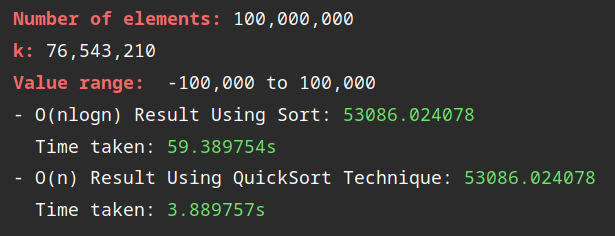
\includegraphics[width=0.7\linewidth]{../images_&_data/kth_smallest/100m} 

}

\caption{\label{fig1:figs}The outputs of the $O(n \log n)$ algorithm using regular sorting and the $O(n)$ QuickSelect algorithm. Number of input elements is $100\,000\,000$ with $k = 76\,543\,210$.}\label{fig:unnamed-chunk-1}
\end{figure}

\hrule

~

~

With the given number of elements, \(k\) and value range, both of the
algorithms produced the same result, which is 53081.606002, but the
running times of them have a significant difference (For the program's
output, see Figure \ref{fig1:figs}).

Since the QuickSelect takes at most \(2n\) running time, the regular
sorting takes at least \(\log(n)/2\) times more than it, and the
\(\log\) is in base 2. In this case, there are \(100\,000\,000\)
numbers, so:
\[\frac{\log(n)}{2} = \frac{\log(100\,000\,000)}{2} \approx 13.2877 \text{ times} \leq \frac{53.615235}{3.588446} \approx 14.9411 \text{ times}\]

Since \(14.9411\) is quite close to \(13.2877\), the running time of
this QuickSelect algorithm in practice is reasonable compared to the
theory.

\hypertarget{section3}{%
\section{\texorpdfstring{3 \enspace Algorithm 2: The refinement of
\(\mathrm{S\pnt{EP}A\pnt{NN}}(S,n,d,\mu,c)\)}{3 Algorithm 2: The refinement of \textbackslash{}mathrm\{S\textbackslash{}pnt\{EP\}A\textbackslash{}pnt\{NN\}\}(S,n,d,\textbackslash{}mu,c)}}\label{section3}}

With the use of the algorithm \textsc{SepAnn$(S,n,d,\mu,c)$}'s output,
this refinement algorithm continues to find an annulus that separates
the points in \(S\) into different smaller sets of points.

Let \(\mu = e\) and \(c = 2(4e)^d\), see {[}1, Remark 1{]}. The
algorithm \textsc{SepAnn$(S,n,d,e,c)$} returns an annulus's center
\(p \in S\) and its radius, \(R'>0\). An input of this refined algorithm
is \(t > 0\), a large enough constant calculated based on \(n\). Let
\(R_i = (1+1/t)^i\cdot R'\), in which \(i\) is a uniformly random
element inclusively from \(1\) to \(t\). The algorithm then finds an
annulus centered at \(p\) with the inner radius \(R_{i-1}\) and outer
radius \(R_{i}\), denoted \(A_i = annulus_S(p, R_{i-1}, R_i)\). If the
annulus contains at most \(n/t\) points then we are done. The algorithm
returns \(p\) and \(R_{i-1}\). This algorithm has the expected \(O(cn)\)
time complexity, see {[}1, Section 3.2{]}. Otherwise, the previous
procedure is repeated until the condition is satisfied. The pseudocode
of this refined algorithm is given below.

\begin{figure}[ht] \centering
  \begin{minipage}{1\linewidth}
    {\LinesNotNumbered
    \begin{algorithm}[H]
    \SetKwInOut{Input}{Input}
    \Input{Let $S$ be a subset of $P$, of size $n \geq 2(4e)^d +1$, $d$ be the space's doubling dimension, $t \geq1$ be an integer.}
    \SetAlgoLined
    \SetKwInOut{Output}{Output}
    \Output{A point $p \in S$ and a radius $R > 0$.}
    \BlankLine

    \centering
    \begin{minipage}{.80\linewidth}
    $c = 2(4e)^d$;

    let $p\in S$ and $R' > 0$ be the output of algorithm \textsc{SepAnn$(S,n,d,e,c)$};

    \Repeat{$s \leq n/t$}
      {$i$ = a uniformly random element in $\{1, 2,\ldots, t\};$

      $R_i = (1+1/t)^i\cdot R'$;

      $R_{i-1} = (1+1/t)^{i-1}\cdot R'$;

      $A_i = annulus_S(p,R_{i-1},R_i)$;

      $s = |A_i|$;
      }
      $R = R_{i-1}$;

      return $p$ and $R$
    \end{minipage}
    \caption{\textsc{SparseSepAnn}$(S,n,d,t)$}
    \end{algorithm}}
  \end{minipage}
  \begin{minipage}{1\textwidth}
    \begin{flushright}
    {\footnotesize \emph{This pseudocode is from [1, Section 3.2]}\par}
    \end{flushright}
  \end{minipage}
\end{figure}

\hypertarget{section4}{%
\section{\texorpdfstring{4 \enspace Algorithm 3: The main closest-pair
algorithm}{4 Algorithm 3: The main closest-pair algorithm}}\label{section4}}

Using the result of \textsc{SparseSepAnn$(S,n,d,t)$}, this main
algorithm \textsc{ClosestPair($S,n,d$)} recursively compute the closest
distance.

Let \(S\) be an \(n\)-sized subset of \(P\), \(d\) be the metric space
\((P, dist)\)'s doubling dimension. In the base case, that is when
\(n < 2(16e)^d\), the algorithm uses brute-force to compute the closest
distance. If this is not the case, the algorithm sets
\(t = \lfloor \frac{1}{16e}(n/2)^{1/d}\rfloor\). This algorithm then
runs \textsc{SparseSepAnn($S,n,d,t$)} with this \(t\) value, and gets
the output \(p \in S\) and \(R>0\) which is the inner radius of the
sparse annulus. The outer radius of it is \((1+1/t)R\).

Let \(S_1\) be the set of points contained in \(ball_S(p, R)\), \(S_2\)
be the set of points contained in \(annulus_S(p, R, (1+1/t)R\) and
\(S_3\) be the set that contains all the points outside of the outer
radius \((1+1/t)R\). This algorithm now recursively calls itself on two
subsets of \(S\) which are points contained in \(ball_S(p,(1+1/t)R)\)
(which is \(S1 \cup S2\)) and outside of \(ball_S(p, R)\) (which is
\(S2 \cup S3\)). Finally, the smaller distance output from two recursive
calls, \(\delta_0 = min(\delta_1, \delta_2)\), is returned. Below is the
algorithm's pseudocode, see {[}1, Section 4.1{]}.

\begin{figure}[ht]
    \centering
    \begin{minipage}{1\linewidth}
      {\LinesNotNumbered
      \begin{algorithm}[H]
      \SetKwInOut{Input}{Input}
      \Input{Let $S$ be a subset of $P$, of size $n \geq 2$, $d$ be the space's doubling dimension.}
      \SetAlgoLined
      \SetKwInOut{Output}{Output}
      \Output{A real number $\delta_0$ satisfies the two properties in [1, Lemma 5].}
      \BlankLine

      \centering
      \begin{minipage}{.86\linewidth}
      \uIf{$n < 2(16e)^d$} {
        $\delta_0$ = the closest-pair distance in $S$ using brute-force;
      }\Else {
        $t = \lfloor \frac{1}{16e}(n/2)^{1/d}\rfloor$;
        
        let $p \in S$ and $R > 0$ be the output of algorithm \textsc{SparseSepAnn($S,n,d,t$)};
        
        $S_1 = ball_S(p,R)$;

        $S_2 = annulus_S(p,R, (1+1/t)R)$;

        $S_3 = S\, \textbackslash\, (S_1 \cup S_2)$;

        $n' = |S_1 \cup S2|$;
        
        $n'' = |S_2 \cup S3|$;

        $\delta'$ = \textsc{ClosestPair($S_1 \cup S_2, n', d$)};

        $\delta''$ = \textsc{ClosestPair($S_2 \cup S_3, n'', d)$};

        $\delta_0 = min(\delta', \delta'')$;
      }
      return $\delta_0$ 
      \end{minipage}
      \caption{\textsc{ClosestPair}$(S,n,d)$}
      \end{algorithm}}
    \end{minipage}
    \begin{minipage}{1\textwidth}
      \begin{flushright}
      {\footnotesize \emph{This pseudocode is from [1, Section 4.1]}\par}
      \end{flushright}
    \end{minipage}
\end{figure}

\hypertarget{section5}{%
\section{\texorpdfstring{5 \enspace The
Implementation}{5 The Implementation}}\label{section5}}

This implementation of the closest-pair doubling algorithm is written in
C++ since it is a very common and fast programming language with
high-level supports of object-oriented programming that can help us
organize the program efficiently (see the implementation's
\href{https://github.com/ThangMinhCao/closestpairdoubling}{\emph{GitHub
repository}}\footnote{GitHub repository of the implementation.
  \href{https://github.com/ThangMinhCao/closestpairdoubling}{\emph{https://github.com/ThangMinhCao/closestpairdoubling}}}
for the source code). The implementation and its components will be
described and explain throughout this section. Also, the code and
description of each function will be given below.

To begin with, a set of points, which does not necessarily refer to
\code{set} in Computer Science, is always one of the input parameters of
each partial algorithm. In this implementation, I would choose
\code{vector}, a very popular built-in data structure of C++. Since its
size can automatically change when we add or remove an element, it is
easy to work with and manage its behavior when implementing. Not only
for storing points, \code{vector} will be used throughout the
implementation to store some other information.

\hypertarget{section5.1}{%
\subsection{5.1 Utility functions and classes}\label{section5.1}}

\hypertarget{section5.1.1}{%
\subsubsection{5.1.1 Random number generator
classes}\label{section5.1.1}}

Due to A. Maheshwari, W. Mulzer and M. Smid, the closest-pair doubling
algorithm uses randomized technique in some parts to find the targets in
linear time. Therefore, generating random numbers is important. I
created two random number generator classes, one for integer and one for
double, to make the program more simple. The generators' code is given
below.

~

\begin{lstlisting}
#include <random>

class RandomInt{
  public:
      RandomInt(int start, int end) 
          : generator{std::random_device{}()}, int_dist(start, end) {}
      int next() { return int_dist(generator); } 

  private:
      std::mt19937 generator;
      std::uniform_int_distribution<> int_dist;
};

class RandomDouble{
  public:
      RandomDouble(int start, int end) 
          : generator{std::random_device{}()}, double_dist(start, end) {}
      double next() { return double_dist(generator); } 

  private:
      std::mt19937 generator;
      std::uniform_real_distribution<> double_dist;
};
\end{lstlisting}
\vspace{-9truemm}
\begin{minipage}{1\textwidth}
  \begin{flushright}
  {\footnotesize \emph{Source \footnotemark: master branch $\rightarrow$ closestpairdoubling/include/RandomGenerator.h }\par}
  \end{flushright}
\end{minipage}
\vspace{0.5truemm}
\footnotetext{Path to the source file in the implementation's GitHub repository.}

~ For each class, I create a uniform distribution with a given range
that corresponds to the number type and an \code{mt19937} random
generator with a \code{random\_device} input. These two variables will
be initialized when a random generator object is instantiated. Each
class also has a \code{next()} function that can be called to return a
random number.

\hypertarget{section5.1.2}{%
\subsubsection{\texorpdfstring{5.1.2 \emph{Point} and \emph{PointList}
classes}{5.1.2  and  classes}}\label{section5.1.2}}

Since points are fundamental elements of the algorithm, and they are not
just numbers (they have their own coordinates), creating a \code{Point}
class is quite essential. Moreover, with the addition of the class
function \code{distance\_to}, the algorithm can calculate the distance
between any two points easily without directly using the points'
coordinates. This function works as the input function \(dist\) that is
provided with the metric space (\(P, dist\)). The implementation code of
the class is given below.

~

\begin{lstlisting}
#include <vector>
#include <cmath>

class Point {
  private:
    std::vector<double> coordinate;
  public:
    explicit Point(std::vector<double> coordinate) {
      this->coordinate = std::move(coordinate);
    }
    Point()= default;
    // distance is calculated using Pythagorean Theorem
    double distance_to(const Point& another_point) {
      double total_square = 0;
      for (int i = 0; i < coordinate.size(); i++) {
        double iDiff = coordinate[i] - another_point.getCoordinate()[i];
        total_square += (iDiff) * (iDiff);
      }
      return sqrt(total_square);
    }
    std::vector<double> getCoordinate() const {
      return coordinate;
    }
}
\end{lstlisting}
\vspace{-9truemm}
\begin{minipage}{1\textwidth}
  \begin{flushright}
  {\footnotesize \emph{Source: master branch $\rightarrow$ closestpairdoubling/include/Point.h}\par}
  \end{flushright}
\end{minipage}
\vspace{0.5truemm}

~ Because there is not only one method to generate points (see the
description later in \protect\hyperlink{section6}{Section 6}), so if all
of them are implemented in the \code{main()}, the function will be quite
huge and complicated. Thus, I created another utility class to make the
code more organized, \code{PointList}. The \code{PointList} class
consists of a \code{vector} named \(points\) that store all the points
in a subset of \(P\) and some point generating functions. This class is
used as subsets of \(P\) and to initialize all the points in \(P\) at
the start of the program.

~

\begin{lstlisting}
#include "Point.h"
#include "RandomGenerator.h"

class PointList {
  public:
    std::vector<Point> points;

    // initializes all points uniformly random, see Section 6 for details 
    void random_initializer(int dimension, int point_num,
                            int coor_start_range, int coor_end_range)
    {
      RandomDouble random_double(coor_start_range, coor_end_range);
      for (int i = 0; i < point_num; i++) {
        std::vector<double> coor;
        // number of coordinates is the dimension value
        for (int j = 0; j < dimension; j++) {
          coor.push_back(random_double.next());
        }
        points.push_back(Point(coor));
      }
    }

    // initializes points in grid, see Section 6 for details 
    void grid_initializer(double dist, int xFactor, int yFactor, int position)
    {
      // the grid starts at coordinates (position, position)
      int y = 0;
      while (y < yFactor) {
        int x = 0;
        while (x < xFactor) {
          std::vector<double> coor;
          coor.push_back(position + (x++) * dist);
          coor.push_back(position + y * dist);
          points.push_back(Point(coor));
        }
        y++;
      }
    }
}
\end{lstlisting}
\vspace{-9truemm}
\begin{minipage}{1\textwidth}
  \begin{flushright}
  {\footnotesize \emph{Source: master branch $\rightarrow$ closestpairdoubling/include/PointList.h}\par}
  \end{flushright}
\end{minipage}

\hypertarget{section5.1.3}{%
\subsubsection{\texorpdfstring{5.1.3 \(K^{th}\) smallest element
finder}{5.1.3 K\^{}\{th\} smallest element finder}}\label{section5.1.3}}

The \(K^{th}\) smallest algorithm has its own class. In this class, I
define a shorter type name \code{DVect} which is
\code{std::vector<double>}. The QuickSelect algorithm is divided into
three functions, the main is \code{get}, and two assistances \code{swap}
and \code{partition}. The function \code{get} returns the \(k^{th}\)
smallest element using QuickSelect, and the other using the normal sort.
Although I only use the QuickSelect technique, I create both to compare
their time complexity, see \protect\hyperlink{section2.2}{Section 2.2}.

~

\newpage

\begin{lstlisting}
#include <vector>

typedef std::vector<double> DVect;

class kth_smallest {
  private:
    static void swap (double *a, double *b);
    static int partition(DVect& distances, int start, int end);

  public:
    // get k-th smallest element with QuickSelect
    static double get(DVect& distances, int start, int end, int k);
    // get k-th smallest element with normal sorting 
    static double get_with_sorting(DVect distances, int k);
};
\end{lstlisting}
\vspace{-9truemm}
\begin{minipage}{1\textwidth}
  \begin{flushright}
  {\footnotesize \emph{Source: master branch $\rightarrow$ closestpairdoubling/include/kth_smallest.h}\par}
  \end{flushright}
\end{minipage}
\vspace{0.5truemm}

~ Due to its simplicity and irrelevant uses (only for testing and
analyzing), the implementation of the normal sorting technique will not
be listed in this report, see the \emph{GitHub repository} for the code.
The following is the implementation code of the QuickSelect algorithm.

~

\begin{lstlisting}
#include "kth_smallest.h"
#include "RandomGenerator.h"

void kth_smallest::swap (double *a, double *b) {
  double temp = *a;
  *a = *b;
  *b = temp;
}

int kth_smallest::partition(DVect& distances, int start, int end) {
  double pivot = distances[end];
  int slow = start;
  int fast = start;
  // moving the smaller elements to the left and larger elements to the right
  while (fast < end) {
    if (distances[slow] > pivot) {
      while (fast < end and distances[fast] > pivot) {
        fast++;
      }
      if (distances[fast] < pivot) {
        swap(&distances[slow], &distances[fast]);
      } else {
        break;
      }
    }
    fast++;
    slow++;
  }
    // swapping the pivot from end back to its original place
  swap(&distances[slow], &distances[end]);
  return slow;
}

double kth_smallest::get(DVect& distances, int start, int end, int k) {
  if (start == end) {return distances[start];}
  //  swapping the random pivot to the end
  RandomInt random_int_gen = RandomInt(start, end);
  swap(&distances[random_int_gen.next()], &distances[end]);
  int cur_pivot = partition(distances, start, end);
  if (k == cur_pivot - start + 1) {
    return distances[cur_pivot];
  } else if (k < cur_pivot - start + 1) {
    return get(distances, start, cur_pivot - 1, k);
  } else {
    return get(distances, cur_pivot + 1, end, k - cur_pivot + start - 1);
  }
}

\end{lstlisting}
\vspace{-9truemm}
\begin{minipage}{1\textwidth}
  \begin{flushright}
  {\footnotesize \emph{Source: master branch $\rightarrow$ closestpairdoubling/src/kth_smallest.cpp}\par}
  \end{flushright}
\end{minipage}
\vspace{0.5truemm}

The function \code{swap(double *a, double *b)} swaps two elements in a
vector by swaps the values at the addresses that the pointers \code{*a}
and \code{*b} point to. Thus, their values in a vector are swapped while
their identities are still the same.

The function \code{partition(DVect\& distances, int start, int end)}
takes the last element in \code{distances} to be the pivot. Then, it
rearranges the vector so that every element smaller and larger than
pivot is to the left and right of it. The technique I use in this
function is creating two pointers \code{fast} and \code{slow}. Both
pointers move towards the end step by step together until
\code{distances[slow]} \textgreater{} \code{pivot}, then it stops. The
\code{fast} keep moving until \code{distances[fast]} \textless{}
\code{pivot}, then the value at two indices are swapped. This procedure
is repeated until the \code{fast} reach the end of the vector The
\code{pivot} is now swapped back to the \code{slow} position, where it
is supposed to be.

A generic call is
\code{get(DVect\& distances, int start, int end, int k)}. It first
checks if the sub-vector has only one element (as well as
\code{start == end}) then returns it. Otherwise, it selects a random
pivot in the vector then swaps it with the last element. Now, the
\code{partition} function is called to return the index of the pivot
after rearranging. The base case is when there are exactly \(k\)
elements from index 0 to the current pivot in the original vector (which
is \code{cur\_pivot - start + 1}), so it is the \(k^{th}\) smallest
element. If there are more than \(k\) elements, the function is
recursively called on the sub-vector to the left of the pivot. If there
are less than \(k\) elements, the function is called on the sub-vector
to the right, but now the \(k\) should be decreased by
\code{cur\_pivot - start + 1}. Due to
\protect\hyperlink{section2.2}{Section 2.2}, this procedure takes
\(O(n)\) time complexity.

\hypertarget{the-2d-algorithm-for-testing}{%
\subsubsection{5.1.4 The 2D algorithm for
testing}\label{the-2d-algorithm-for-testing}}

In the project, I also implement the 2D closest-pair algorithm using
Divide-and-conquer algorithm due to Bentley and Shamos, see {[}5{]}.
This algorithm is very helpful in testing and debugging the closest-pair
doubling algorithm because of its short running time. I will briefly
describe the algorithm below.

Given a set of point \(P\), the base case is when \(P\) contains less
than 2 points. If there is only one, the algorithm returns positive
\(\infty\). If there are two points, the algorithm basically returns the
distance between them. Otherwise, \(P\) is sorted in ascending order
based on the points' \(x\)-coordinate. Then, it chooses a vertical line,
\(\ell\), that divides the set \(P\) into two halves, \(P_1\) contains
\(\lfloor n/2 \rfloor\) points and \(P_2\) contains
\(\lceil n/2 \rceil\) points. The algorithm now recursively calls itself
on \(P_1\) and \(P_2\), so the minimum of the two outputs would be the
temporary closest-pair distance, \(\delta_0 = min(\delta_1, \delta_2)\).
It is obvious that there could be a pair of points (one from \(P_1\) and
the other from \(P_2\)) which has a closer distance than the temporary
\(\delta_0\).

To combine the two set \(P_1\) and \(P_2\), we create a strip centered
at \(\ell\) with its left end and right end are the lines \(\ell_1\) and
\(\ell_2\) so that both lines are \(\delta_0\) away from \(\ell\). All
the points in the strip are now sorted based on their \(y\)-coordinate.
The algorithm then can loop through the strip and check if there is any
smaller distance than \(\delta_0\). Fortunately, for each point in the
strip, the algorithm just needs to check the distances between the
current point with its 7 successive points, that have \(y\)-coordinates
\(\geq\) the current point's \(y\)-coordinate. If there is any closer
distance, it is assigned to \(\delta_0\). Finally, \(\delta_0\) is
returned.

To keep the report on point and less complicated, the code of this 2D
algorithm will not be listed. See the implementation on my
\href{https://github.com/ThangMinhCao/closestpairdoubling/tree/master/utils}{\emph{GitHub
repository}}\footnote{The implementation of the 2D algorithm with merge
  sort algorithm.
  \href{https://github.com/ThangMinhCao/closestpairdoubling/tree/master/utils}{\emph{https://github.com/ThangMinh-}
  \emph{Cao/closestpairdoubling/tree/master/utils}}}.

\hypertarget{section5.2}{%
\subsection{5.2 The closest-pair doubling algorithm}\label{section5.2}}

The implementation of the closest-pair algorithm still consists of three
main functions, \code{sep\_ann}, \code{sparse\_sep\_ann} and
\code{closest\_pair}. Moreover, the \code{brute\_force} function is
added to be used in the base case. The following is the algorithm's
class.

~

\begin{lstlisting}
#include "PointList.h"

typedef std::vector<double> DVect;

class ClosestPairDoubling {
  private:
    static std::tuple<Point, double, DVect>
                sep_ann(PointList &S, int n, double mu, double c);
    static std::pair<Point, double>
                sparse_sep_ann(PointList &S, int n, double d, int t);
  public:
    ClosestPairDoubling() = default;
    static double brute_force(PointList &S);
    static double closest_pair(PointList &S, double d, int recursion=0);
};
\end{lstlisting}
\vspace{-9truemm}
\begin{minipage}{1\textwidth}
  \begin{flushright}
  {\footnotesize \emph{Source: master branch $\rightarrow$ closestpairdoubling/include/ClosestPairDoubling.h}\par}
  \end{flushright}
\end{minipage}

\hypertarget{section5.2.1}{%
\subsubsection{\texorpdfstring{5.2.1 The
\(\mathrm{S\pnt{EP}A\pnt{NN}}(S,n,d,\mu,c)\)
algorithm}{5.2.1 The \textbackslash{}mathrm\{S\textbackslash{}pnt\{EP\}A\textbackslash{}pnt\{NN\}\}(S,n,d,\textbackslash{}mu,c) algorithm}}\label{section5.2.1}}

The \code{sep\_ann} function starts by defining some important variables
to be used in its loop. Let \code{p} be the chosen random point in
\(S\), \code{Rp} be the radius of the smallest ball containing at least
\(n/c\) points, \code{distances\_from\_p} be the vector stores the
distances between \(p\) and all points in \(S\) and
\code{outer\_ball\_count} be the number of points in the outer ball,
\(ball_S(p,\mu R_p)\). To select a random point \(p\), I initialize an
integer random generator \code{int\_gen} with the range from 0 to
\(n - 1\), possible indices of points in \(S\).

Since \(c\) is calculated based on \(d\) which could be done outside the
function, I removed the input \(d\) of the \code{sep\_ann} function.

~

\begin{lstlisting}
std::tuple<Point, double, DVect>
      ClosestPairDoubling::sep_ann(PointList &S, int n, double mu, double c)
{
  Point p;
  double Rp = -1.0;
  DVect distances_from_p;
  int outer_ball_count = (n / 2) + 1;
  RandomInt int_gen(0, n - 1);

  while (Rp == -1.0 or outer_ball_count > std::floor(n / 2)) {
    distances_from_p.clear();

    // selecting the random point p and calculate all the distances
    int random_index = int_gen.next();
    p = S.points[random_index];
    for (const Point& point: S.points) {
      distances_from_p.push_back(p.distance_to(point));
    }
    Rp = kth_smallest::get(distances_from_p, 0,
                            (int)distances_from_p.size(), ceil(n / c));

    // counting the number of point in the outer ball
    outer_ball_count = 0;
    for (double dist: distances_from_p) {
      if (dist <= mu * Rp) {
        outer_ball_count++;
      }
    }
  }
  return std::make_tuple(p, Rp, distances_from_p);
}
\end{lstlisting}
\vspace{-9truemm}
\begin{minipage}{1\textwidth}
  \begin{flushright}
  {\footnotesize \emph{Source: master branch $\rightarrow$ closestpairdoubling/src/ClosestPairDoubling.cpp}\par}
  \end{flushright}
\end{minipage}
\vspace{0.5truemm}

Each time the \(while\) loop is repeated, \code{distances\_from\_p} is
cleared to get rid of the previous loop's result. The function uses
\code{int\_gen} to generate a random point in \(S\), then it stores
distances between \(p\) and every point in \(S\) including itself into
\code{distances\_from\_p}. The QuickSelect function from
\code{kth_smallest} class is now used to get the \(ceil(n/c)\)-smallest
element in \code{distances\_from\_p}, then it is assigned to \code{Rp}.
The function loops through the distance vector to count the number of
points inside the outer ball and assigns it to
\code{outer\_ball\_count}. If \code{outer\_ball\_count} \textless{}
\(\lfloor n/2 \rfloor\) then we are done, the function returns a tuple
containing \code{p}, \code{Rp} and \code{distances\_from\_p}. If this is
not the case, the procedure is repeated until the condition is
satisfied. Note that, I return \code{distances\_from\_p} here to use it
in \textsc{SparseSepAnn} without spending time to loop through the
vector again.

\hypertarget{section5.2.2}{%
\subsubsection{\texorpdfstring{5.2.2 The refined algorithm
\(\mathrm{S\pnt{PARSE}S\pnt{EP}A\pnt{NN}}(S,n,d,t)\)}{5.2.2 The refined algorithm \textbackslash{}mathrm\{S\textbackslash{}pnt\{PARSE\}S\textbackslash{}pnt\{EP\}A\textbackslash{}pnt\{NN\}\}(S,n,d,t)}}\label{section5.2.2}}

Let \code{sep\_ann\_res} be the output of the function
\code{sep\_ann(S, n, e, c)}, \code{Ai\_size} be the number of points
\(annulus_S(p, R_{i-1}, R_i)\) contains. Let \code{p}, \code{R\_prime}
and \code{distance\_from\_p} be the variables store the values which are
derived from \code{sep\_ann\_res}. The implementation code of
\textsc{SparseSepAnn} is given below.

~

\begin{lstlisting}
std::pair<Point, double>
  ClosestPairDoubling::sparse_sep_ann(PointList &S, int n, double d, int t)
{
  const double e = std::exp(1.0); // the Euler constant
  double c = 2 * pow(4 * e, d);
  std::tuple<Point, double, DVect> sep_ann_res = sep_ann(S, n, e, c);

  // followings are results derived from sep_ann_res
  Point p = std::get<0>(sep_ann_res);
  double R_prime = std::get<1>(sep_ann_res);
  DVect distances_from_p = std::get<2>(sep_ann_res);

  int Ai_size = n / t + 1;
  RandomInt range_t_random(1, t);

  double R;
  while (Ai_size > n / t) {
    int random_i = range_t_random.next();
    double Ri = pow(1 + 1.0 / t, random_i) * R_prime;
    R = pow(1 + 1.0 / t, random_i - 1) * R_prime;
    Ai_size = 0;
    for (double dist: distances_from_p) {
      if (R <= dist and dist <= Ri) {
        Ai_size++;
      }
    }
  }
  return std::pair<Point, double> {p, R};
}
\end{lstlisting}
\vspace{-9truemm}
\begin{minipage}{1\textwidth}
  \begin{flushright}
  {\footnotesize \emph{Source: master branch $\rightarrow$ closestpairdoubling/src/ClosestPairDoubling.cpp}\par}
  \end{flushright}
\end{minipage}
\vspace{0.5truemm}

The algorithm first selects a random value \(i\) in the range from 1 to
\(t\) using the random generator \code{range\_t\_random}, then it
calculates the inner and outer radius of \(annulus_S(p, R_{i-1}, R_i)\)
in which \(R_i = (1+1/t)^i\). An inner \code{for} loop goes through
\code{distance\_from\_p} to count the number of points in the annulus
and then stores the number to \code{Ai\_size}. If \code{Ai\_size}
\textgreater{} \(n/t\), the right annulus is found, then it returns
\code{p} and \code{R}. Otherwise, the \code{while} loop repeats the
procedure to find the annulus that satisfies \code{Ai\_size}
\(\leq n/t\).

\hypertarget{section5.2.3}{%
\subsubsection{\texorpdfstring{5.2.3 The main closest-pair algorithm
\(\mathrm{C\pnt{LOSEST}P\pnt{AIR}}(S,n,d)\)}{5.2.3 The main closest-pair algorithm \textbackslash{}mathrm\{C\textbackslash{}pnt\{LOSEST\}P\textbackslash{}pnt\{AIR\}\}(S,n,d)}}\label{section5.2.3}}

Let \code{n} be the number of points contained in \(S\), \code{e} be the
Euler constant, \code{delta0} be the closest-pair distance in \(S\).
Furthermore, I combine the three subsets \(S_1\), \(S_2\) and \(S_3\)
(see \protect\hyperlink{section4}{Section 4}) to only two that are
\code{S1orS2} and \code{S2orS3} that represent the subset
\(S_1 \cup S_2\) and \(S_2 \cup S_3\).

~

\begin{lstlisting}
double
    ClosestPairDoubling::closest_pair(PointList &S, double d, int recursion)
{
  int n = (int)S.points.size();
  const double e = std::exp(1.0);
  double delta0; // the closest-pair distance in S

  if (n < 2 * pow(16 * e, d)) {
    return brute_force(S);
  } else {
    int t = floor((1 / (16 * std::exp(1.0))) * pow((double)n / 2, 1 / d));
    std::pair<Point, double> ssann_result = sparse_sep_ann(S, n, d, t);
    Point p = ssann_result.first;
    double R = ssann_result.second;
    PointList S1orS2 = PointList();
    PointList S2orS3 = PointList();
    for (const Point& point: S.points) {
      double d_to_p = p.distance_to(point);
      if (d_to_p <= R) {
        S1orS2.points.push_back(point);
      } else if (d_to_p > R and d_to_p <= (1 + 1.0/t) * R) {
        S1orS2.points.push_back(point);
        S2orS3.points.push_back(point);
      } else {
        S2orS3.points.push_back(point);
      }
    }
    std::vector<Point>().swap(S.points); // free the memory that stores S
    double delta1 = closest_pair(S1orS2, d, ++recursion);
    double delta2 = closest_pair(S2orS3, d, ++recursion);
    delta0 = std::min(delta1, delta2);
  }
  return delta0;
}
\end{lstlisting}
\vspace{-9truemm}
\begin{minipage}{1\textwidth}
  \begin{flushright}
  {\footnotesize \emph{Source: master branch $\rightarrow$ closestpairdoubling/src/ClosestPairDoubling.cpp}\par}
  \end{flushright}
\end{minipage}
\vspace{0.5truemm}

With \(t = \lfloor \frac{1}{16e}(n/2)^{1/d}\rfloor\),
\code{sparse\_sep\_ann(S,b,d,t)} is called, and the outputs of it are
assigned into \code{p} and \code{R}. The \code{for} loop goes through
\(S\) to build the two sets by adding corresponding points to them using
the distance from \(p\) to each point. Let \code{d\_to\_p} be the
distance from \(p\) to the current point in the \code{for} loop. If
\code{d\_to\_p} \(\leq\) \(R\), the current point is in the
\(ball_S(p, R)\), so it is added to \code{S1orS2}. If \(R <\)
\code{d\_to\_p} \(\leq (1 + 1/t)R\), the point is in the
\(annulus_S(p, R, (1+1/t)R)\), then it is added to both \code{S1orS2}
and \code{S2orS3}. Otherwise, the point is appended into only
\code{S2orS3} since it is outside the outer radius.

Because every point in \(S\) is now in \code{S1orS2} and \code{S2orS3},
it is not necessary to keep the vector \code{S} as well as its memory
usage, which could be stacked up after many recursive calls and cause
memory overload. Thus, after storing all the points into \code{S1orS2}
and \code{S2orS3}, I clear the vector \code{S} and its data in the
memory using the function \code{vector::swap()} to swap \code{S} with an
empty vector. Note that, I will make sure to pass the full set of points
\textbf{by value} or pass a copy of it to the first call of the
algorithm, so the original one will not be changed. Therefore, it can
not affect the execution of \code{brute\_force} for testing later.

After that, the outputs of two recursive calls, one on \code{S1orS2} and
one on \code{S2orS3}, will be stored in \code{delta1} and \code{delta2}
variables. Finally, the smaller one of them will be assigned into
\code{delta0} and returned.

\hypertarget{section5.3}{%
\subsection{5.3 The closest-pair distance of non-Euclidean
spaces}\label{section5.3}}

The algorithm runs correctly in a special case in which the given metric
space is non-Euclidean of doubling dimension 1, see {[}3, Section 2.1{]}
for more details. Given a metric space \(S = \{p_1, p_2,\ldots,p_n\}\)
that contains \(n\) ``points'', denoted \(p_m\) with
\(1 \leq m \leq n\). Specifically, the value of \(p_m\) represents an
integer between a given range. Let \(i\) and \(j\) be any number that
satisfies \(1 \leq i \leq j \leq n\), the distance between \(p_i\) and
\(p_j\) is defined:

\[
  dist(p_i, p_j) =
  \begin{cases}
  0 & \text{if $i=j$} \\
  4^{max(i,j)} & \text{if $i\neq j$} \\
  \end{cases}
\]

Using the definition, the closest-pair algorithm finds the closest
distance in this metric space normally without changing any core detail.

Although the points are just integers, I still treat them as
\code{Point} objects with 1D coordinates. Therefore, I do not need to
make many small changes which may lead to programming errors that can
take a lot of time to fix, and I still keep the main idea of the
algorithm that works with the \code{Point} class.

The only problem is that the distance between any two points could be
extremely large. For instance, let the upper bound of the points' value
be a big number, say 100, so \(p_i \leq p_j \leq 100\). Let
\(p_i = 100\), then \(dist(p_i,p_j)=4^{100} > 1.6 \times 10^{60}\) which
is much larger than the maximum 32-bit integer that C++ can handle.
Therefore, I decided to use a library named
\href{https://www.boost.org/}{\emph{Boost}}\footnote{The \emph{Boost}
  library's website.
  \href{https://www.boost.org/}{\emph{https://www.boost.org/}}} which
can handle numbers with precisions up to 1024 bits. When changing the
current algorithm to use \emph{Boost}, I only need to replace the
\code{double} type of normal distances by \code{cpp\_int} type which can
automatically choose the corresponding precision for each distance.
Also, I needed to make some minor changes, so the algorithm can be able
to run correctly. Since there are not many changes and they do not
affect the main theory of the algorithm, the implementation for this
non-Euclidean will not be listed in this report. See the
\href{https://github.com/ThangMinhCao/closestpairdoubling/tree/strange_metric}{\code{strange\_metric}
branch}\footnote{The implementation of the algorithm on non-Euclidean
  metrics.
  \href{https://github.com/ThangMinhCao/closestpairdoubling/tree/strange_metric}{\emph{https://github.com/ThangMinhCa}
  \emph{o/closestpairdoubling/tree/strange\_metric}}} of my GitHub
repository for the implementation.

\hypertarget{section6}{%
\section{\texorpdfstring{6 \enspace The practical running time and
behavior}{6 The practical running time and behavior}}\label{section6}}

After doing many tests on normal Euclidean spaces, I found out that the
algorithm's behavior is different based on the way the points are
arranged on the metric space. There are two approaches to generate the
points that give me the most obvious differences.

\begin{enumerate}
\def\labelenumi{\arabic{enumi}.}
\item
  \textbf{Generating uniformly random} points spread throughout the
  space. To do this, we can just use any of the random number generators
  to get the points' random coordinates in a given range, see
  \protect\hyperlink{section5.1.1}{Section 5.1.1} and
  \protect\hyperlink{section5.1.2}{Section 5.1.2} for more details.
\item
  \textbf{Generating points evenly in a grid}. Let \(n\) be the number
  of points, \(a\) and \(b\) be any two factors of \(n\) that satisfies
  \(a\times b = n\), \(d\) be the distances between any two points which
  are close together. Start at any position, the points are set into the
  \(a \times b\) grid which means each point is on a corner of a
  \(d\)-sided square, see Figure \ref{fig:grid}.
\end{enumerate}

\vspace{-2truemm}
\begin{figure}[!h]
\centering
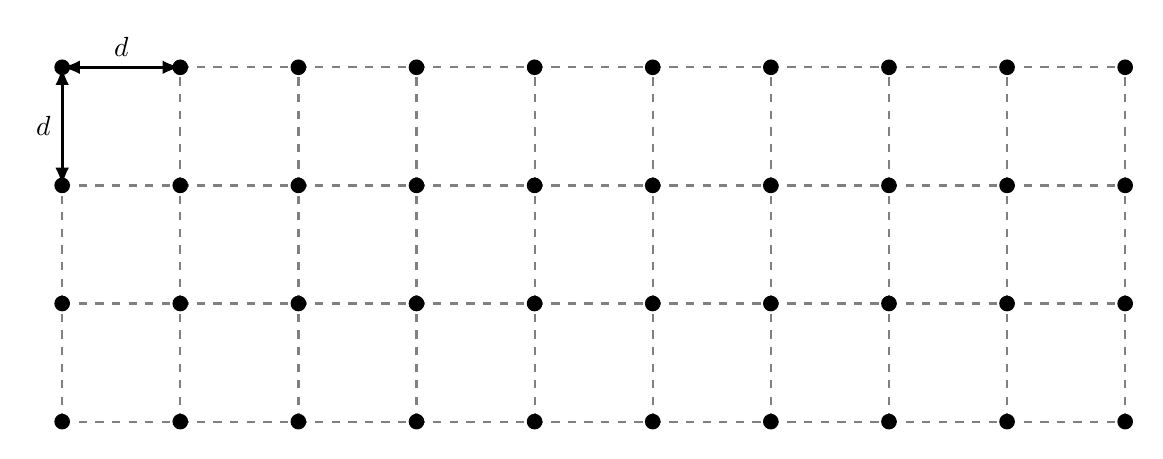
\begin{tikzpicture}
  \foreach \x in {0, 1, 2, 3, 4, 5, 6,7,8,9} {
    \foreach \y in {0, 1, 2, 3} {
      \node (thisNode) at (1.5*\x, 1.5*\y) {};
      \ifthenelse{\x=9}{}{\draw[dashed,gray,thick] (1.5*\x,1.5*\y) -- (1.5*\x+1.5, 1.5*\y);}
      \ifthenelse{\y=3}{}{\draw[dashed,gray,thick] (1.5*\x,1.5*\y) -- (1.5*\x, 1.5*\y+1.5);}
      \node at (thisNode) [circle,fill=black,inner sep=2pt] {};
    }
  }
  \draw[black,very thick,latex-latex] (0, 1.5*3) -- node[above] {$d$} (1.5, 1.5*3);
  \draw[black,very thick,latex-latex] (0, 1.5*3) -- node[left] {$d$} (0, 1.5*2);
\end{tikzpicture}

\caption{An example of points in a grid on a Euclidean space. A set of 40 points that gives us a $4\times10$ grid. Points are placed at corners of the squares whose sides are equal to $d$ that could be any number.}
\label{fig:grid}
\end{figure}

\hrule

~

~

Since the points in non-Euclidean spaces are simply integers, they do
not have properties as many as the ones on normal Euclidean ones.
Therefore, different ways to generate points do not change its behavior
which is already as expected. I will only show its behavior with random
points, see \protect\hyperlink{section6.2}{Section 6.2}.

To generate random points in a non-Euclidean space, I use a
\code{RandomInt} object. With a given range and number of points, I can
easily call \code{next()} to get a value to initialize a \code{Point}
and store it into a \code{PointList} object.

\hypertarget{the-practical-running-time}{%
\subsection{6.1 The practical running
time}\label{the-practical-running-time}}

To correctly compare the algorithm's running time, we can use
brute-force which takes \(O(n)\) time or the 2D algorithm for only 2D
points. However, to have the running time that is close to the theory,
the number of points in \(P\) must be extremely large since the base
case of the algorithm is when \(n < 2(16e)^d\), which is already a quite
large number (approximately \(79\,550\) points in 2D and more than
\(3\,000\,000\) points in 3D, for example). The algorithm could take
days to finish calculating the whole metric space, and in this case,
brute-force would take a lot more than that amount of time, which is not
very reasonable for me to keep the program running until it finishes.
Fortunately, since the running time of the algorithm is \(O(n\log n)\)
which is in theory and also expected in practice, the ratio of the
actual running time (in seconds) to the theoretical should be
approximately the same for different large enough numbers of points.
Thus, we can use this information to prove that the running time in
practice is actually \(O(n\log n)\).

Particularly, let \(n\) be the number of points in a metric space,
denoted \(|P|\), \(m\) be a number which is much larger than the base
case of the algorithm (\(2(16e)^{\log_27} \approx 79550\) points in 2D
metric spaces), \(r_n\) be the ratio of the actual running time to the
theoretical one that is calculated using \(n\) with the \(\log\) of base
2. I would initialize and run the algorithm on different metric spaces
\(P\) with \(n \in sizes = \{m, 2m, 4m, 8m, 16m\}\). For each size, I
would run the algorithm several times to find the average running time,
denoted \(T(n)\).

Having \(n\) and \(T(n\)), the ratio is calculated as below:
\[r_n = \frac{T(n)}{n\log n}\]

As expected, the ratios should be approximately the same. Denoted:
\[r_m \approx r_{2m} \approx r_{4m} \approx r_{8m} \approx r_{16m}\]

If this holds, the practical running time represents \(O(n\log n)\)
time. This is obvious because they have the same time complexity, so
when the actual amount of time changes by an amount, the theoretical one
should change by the same amount that is also based on the number of
points.

After running the algorithm with different kinds of inputs, the tables
and graphs below are the results that I come up with.

\begin{enumerate}
\def\labelenumi{\arabic{enumi}.}
\tightlist
\item
  \textbf{Random generated Euclidean metric spaces:} I choose
  \(m = 500\,000\) points since it is much bigger than the base case,
  and as I estimated, the algorithm would take a reasonable time to
  finish all cases.
\end{enumerate}

\begin{figure}
\centering
\begin{minipage}{1\textwidth}
  \centering
    \begin{tabularx}{\textwidth}{|>{\centering\arraybackslash}X|>{\centering\arraybackslash}X|>{\centering\arraybackslash}X|>{\centering\arraybackslash}X|>{\centering\arraybackslash}X|>{\centering\arraybackslash}X|}
  \hline
  \multirow{2}{*}{$\boldsymbol n$} & \multicolumn{4}{c|}{\textbf{The running time (in seconds)}} & \multirow{2}{*}{$\boldsymbol{r_n = \frac{T(n)}{n\log n}}$}\\
    \cline{2-5}
           & $T_1$   & $T_2$    & $T_3$    & $\boldsymbol{T(n)}$ &    \\ \hline
   $500\,000$  & 2176.5  & 2237.33  & 2211.71  & 2208.51   & $2.333\times 10^{-4}$ \\ \hline
  $1\,000\,000$  & 3047.94 & 3063     & 3091.8   & 3067.58   & $1.539\times 10^{-4}$ \\ \hline
  $2\,000\,000$  & 6280.73 & 6040.06  & 5844.34  & 6055.04   & $1.446\times 10^{-4}$ \\ \hline
  $4\,000\,000$  & 12888.7 & 12761.5  & 12632.7  & 12760.97  & $1.454\times 10^{-4}$ \\ \hline
  $8\,000\,000$  & 33400.4 & 32850.6  & 31038.6  & 32429.8   & $1.767\times 10^{-4}$ \\ \hline
  \end{tabularx}
\end{minipage}
\caption[Caption]{The table of random points metric spaces' data of running time and the ratio $r_n$.}
\label{fig:randomdata}
\end{figure}

\hrule

~

\begin{figure}
\begin{minipage}{0.95\textwidth}
\begin{center}
\begin{tikzpicture}
  \begin{axis}[ 
    height=5.7cm,
        width=12.7cm,
    minor tick num=5,
    grid=both,
    grid style={line width=.1pt, draw=gray!20},
    major grid style={line width=.2pt,draw=gray!40},
    ymin=0.0001,
        ymax=0.00028,
    xlabel=$n$,
    ylabel={$r_n$},
        ylabel style={rotate=-90}
  ] 
        \addplot file[skip first] {random_data.txt};
  \end{axis}
\end{tikzpicture}
\end{center}
\end{minipage}
\caption[Caption]{The graph of ratios $r_n$ versus different values of $n$ of random points with $n \in \{500\,000, 1\,000\,000, 2\,000\,000, 4\,000\,000, 8\,000\,000\}$ (with y-interval = $0.5\times10^{-4}$).}
\label{fig:randomgraph}
\end{figure}
\hrule

As you can see in the table (see Figure \ref{fig:randomdata}), for
random points, the ratios \(r_n\) do not have any significant
differences. By assigning them the same base and exponent of their
scientific notation (\(10^{-4}\)), their coefficients are mostly the
same except for the \(500\,000\) points, which is still less than double
of the lowest ratio. This is reasonable since many factors that can
affect the running time of the program. Also, this is the lowest value
of \(n\) in the set, so its running time probably has the highest error.
The graph also shows that the points are roughly on a horizontal line,
so the ratios have acceptable differences, see Figure
\ref{fig:randomgraph}.

\begin{enumerate}
\def\labelenumi{\arabic{enumi}.}
\setcounter{enumi}{1}
\tightlist
\item
  \textbf{Grid generated Euclidean metric spaces:} I choose
  \(m = 200\,000\) points in this case because the algorithm
  \textsc{SepAnn} will repeat several times most of the time it is
  called, which leads to much longer running time. Also, that is still a
  good number which is about 2.5 times larger than the base case, so it
  probably returns a good result of running time.
\end{enumerate}

\begin{figure}
\centering
\begin{minipage}{1\textwidth}
  \centering
    \begin{tabularx}{\textwidth}{|>{\centering\arraybackslash}X|>{\centering\arraybackslash}X|>{\centering\arraybackslash}X|>{\centering\arraybackslash}X|>{\centering\arraybackslash}X|>{\centering\arraybackslash}X|}
  \hline
  \multirow{2}{*}{$\boldsymbol n$} & \multicolumn{4}{c|}{\textbf{The running time (in seconds)}} & \multirow{2}{*}{$\boldsymbol{r_n = \frac{T(n)}{n\log n}}$}\\
    \cline{2-5}
           & $T_1$   & $T_2$    & $T_3$    & $\boldsymbol{T(n)}$ &    \\ \hline
   $200\,000$  & 3467.18  & 3191.12  & 3242.48  & 3304.22   & $0.938\times 10^{-3}$ \\ \hline
  $400\,000$  & 8107.99 & 8298.77  & 8787.8   & 8398.18   & $1.128\times 10^{-3}$ \\ \hline
  $800\,000$  & 19771.3 & 18744.3  & 19015.7  & 19177.1  & $1.222\times 10^{-3}$ \\ \hline
  $1\,600\,000$  & 38205.9 & 36618.35  & 39131.24  & 37993.08  & $1.152\times 10^{-3}$ \\ \hline
  $3\,200\,000$  & 86249.05 & 83354.21  & 82318.96 & 83974.07  & $1.214\times 10^{-3}$ \\ \hline
  \end{tabularx}
\end{minipage}
\caption[Caption]{The table of grid points metric spaces' data of running time and the ratio $r_n$.}
\label{fig:griddata}
\end{figure}

\hrule

~

\begin{figure}
\begin{minipage}{0.95\textwidth}
\begin{center}
\begin{tikzpicture}
  \begin{axis}[ 
    height=5cm,
        width=13cm,
    minor tick num=5,
    grid=both,
    grid style={line width=.1pt, draw=gray!20},
    major grid style={line width=.2pt,draw=gray!40},
    ymin=0,
        ymax=0.0025,
    xlabel=$n$,
    ylabel={$r_n$},
        ylabel style={rotate=-90}
  ] 
        \addplot file[skip first] {grid_data.txt};
  \end{axis}
\end{tikzpicture}
\end{center}
\end{minipage}
\caption[Caption]{The graph of ratios $r_n$ versus different values of $n$ of grid points with $n \in \{200\,000, 400\,000, 800\,000, 1\,600\,000, 3\,200\,000\}$ (with y-interval = $10^{-3}$).}
\label{fig:gridgraph}
\end{figure}

\hrule

~

~

The relationship is clearer in this example of grid generated points.
All the ratios are very close to each other, see \(r_n\) column of
Figure \ref{fig:griddata}. The graph also shows that the differences
between the ratios are very small since all the points are almost on a
horizontal line.

\begin{enumerate}
\def\labelenumi{\arabic{enumi}.}
\setcounter{enumi}{2}
\tightlist
\item
  \textbf{Random generated non-Euclidean metric spaces:} Since handling
  extremely large numbers makes the program significantly slower, I
  start with a much smaller value of \(m\) (\(2\,000\) points) compared
  to the Euclidean spaces. However, for non-Euclidean spaces, the
  doubling dimension is 1, so the base case is approximately 87 points.
  Thus, \(2\,000\) is a pretty large number of point compared to the
  base case.
\end{enumerate}

\begin{figure}
\centering
\begin{minipage}{1\textwidth}
  \centering
    \begin{tabularx}{\textwidth}{|>{\centering\arraybackslash}X|>{\centering\arraybackslash}X|>{\centering\arraybackslash}X|>{\centering\arraybackslash}X|>{\centering\arraybackslash}X|>{\centering\arraybackslash}X|}
  \hline
  \multirow{2}{*}{$\boldsymbol n$} & \multicolumn{4}{c|}{\textbf{The running time (in seconds)}} & \multirow{2}{*}{$\boldsymbol{r_n = \frac{T(n)}{n\log n}}$}\\
    \cline{2-5}
           & $T_1$   & $T_2$    & $T_3$    & $\boldsymbol{T(n)}$ &    \\ \hline
   $2000$  & 10.3557  & 8.83033  & 6.09795  & 8.428  & $3.843\times 10^{-4}$ \\ \hline
  $4000$  & 38.6867 & 47.721  & 34.8211   & 40.4096 & $8.443\times 10^{-4}$ \\ \hline
  $8000$  & 209.766 & 257.704  & 217.096  & 228.1886  & $2.2\times 10^{-3}$ \\ \hline
  $16000$  & 1439.05 & 1202.57 & 1173.77  & 1271.4633  & $5.69\times 10^{-3}$ \\ \hline
  $32000$  & 7692.18 & 7825.26  & 7718.64  & 7745.36  & $1.617\times 10^{-2}$ \\ \hline
  \end{tabularx}
\end{minipage}
\caption[Caption]{The table of random points non-Euclidean metric spaces' data of running time and the ratio $r_n$.}
\label{fig:randomdata}
\end{figure}

\hrule

~

\begin{figure}
\begin{minipage}{0.95\textwidth}
\begin{center}
\begin{tikzpicture}
  \begin{axis}[ 
    height=8cm,
        width=14cm,
    minor tick num=5,
    grid=both,
    grid style={line width=.1pt, draw=gray!20},
    major grid style={line width=.2pt,draw=gray!40},
    ymin=0,
        ymax=0.02,
    xlabel=$n$,
    ylabel={$r_n$},
        ylabel style={rotate=-90}
  ] 
        \addplot file[skip first] {non_Eu_data.txt};
  \end{axis}
\end{tikzpicture}
\end{center}
\end{minipage}
\caption[Caption]{The graph of ratios $r_n$ versus different values of $n$ of random points on non-Euclidean spaces with $n \in \{2000, 4000, 8000, 16\,000, 32\,000\}$ (with y-interval = $0.5\times10^{-2}$).}
\label{fig:randomgraph}
\end{figure}

\hrule

~

~

\hypertarget{section6.2}{%
\subsection{\texorpdfstring{6.2 Probability to select a ``good'' point
of
\(\mathrm{S\pnt{EP}A\pnt{NN}}(S,n,d,\mu,c)\)}{6.2 Probability to select a ``good'' point of \textbackslash{}mathrm\{S\textbackslash{}pnt\{EP\}A\textbackslash{}pnt\{NN\}\}(S,n,d,\textbackslash{}mu,c)}}\label{section6.2}}

Again, the goal of algorithm \textsc{SepAnn($S,n,d,\mu,c$)} is to find a
``good'' point \(p\) in \(S\). A ``good'' point \(p\) implies that with
\(R_p\) (the radius of the smallest \(ball_S(p,R_p)\) that contains at
least \(n/c\) points), the \(ball_S(p,\mu R_p)\) contains at most
\(n/2\) points. Due to A. Maheshwari, W. Mulzer and M. Smid {[}1, Lemma
3{]}, the algorithm has probability at least \(1/c\) (about \(1/1623.4\)
in 2D space) to select a good point uniformly random from \(S\). Like
the practical running time, the number of times the algorithm
\textsc{SepAnn($S,n,d,\mu,c$)} repeats until it gets a good point also
depends on the way how the input points are generated. This only applies
the normal Euclidean metric spaces.

Generating point randomly produces a surprising behavior of this
algorithm. Every time \textsc{SepAnn($S,n,d,\mu,c$)} is called, it only
repeats \emph{once} until it gets to the base case, that means the
probability to get a good point is 100\%, see algorithm's data on
\href{https://github.com/ThangMinhCao/closestpairdoubling/blob/master/report/images_\%26_data/closest_pair/random_generation/random_sep_ann_data.txt}{\emph{GitHub
repository}}\footnote{Random points SepAnn data.
  \href{https://github.com/ThangMinhCao/closestpairdoubling/blob/master/report/images_\%26_data/closest_pair/random_generation/random_sep_ann_data.txt}{\emph{https://github.com/ThangMinhCao/closestpairdoubling/blob/master/rep
  ort/images}\_\%\emph{26\_data/closest\_pair/random\_generation/random\_sep\_ann\_data.txt}}}.
Since the points are generated randomly, so they change every time,
there are no explanations about specific properties of the points in
this case. However, since \(100\%\) satisfied the probability at least
\(1/c\), this result is reasonable.

On the other hand, when using the grid way to generate points, the
algorithm \textsc{SepAnn($S,n,d,\mu,c$)} now repeats multiple times
which is its expected behavior, see an example output in Figure
\ref{fig:data}. Again, the lowest probability in most of the trials in
this case is about \(1/20\) which satisfies probability at least
\(1/c\). For the full grid input data, see the
\href{https://github.com/ThangMinhCao/closestpairdoubling/blob/master/report/images_\%26_data/closest_pair/grid_generation/grid_sepann_data.txt}{\emph{GitHub
repository}}\footnote{Grid points SepAnn data.
  \href{https://github.com/ThangMinhCao/closestpairdoubling/blob/master/report/images_\%26_data/closest_pair/grid_generation/grid_sepann_data.txt}{\emph{https://github.com/ThangMinhCao/closestpairdoubling/blob/master/report/}
  \emph{images}\_\%\emph{26\_data/closest\_pair/grid\_generation/grid\_sepann\_data.txt}}}.

\begin{figure}
\begin{minipage}{0.48\textwidth}
  \centering
  \begin{tabular}{|c|c|}
  \hline
  $\boldsymbol n$   & \textbf{Repeat times} \\ \hline
   200000  & 6            \\ \hline
   193836  & 7            \\ \hline
   179534  & 2            \\ \hline
   172501  & 1            \\ \hline
   158381  & 13           \\ \hline
   156531  & 3            \\ \hline
  \ldots   & \ldots       \\ \hline
  \end{tabular}
\end{minipage}
\begin{minipage}{0.48\textwidth}
  \centering
  \begin{tabular}{|c|c|}
  \hline
  $\boldsymbol n$   & \textbf{Repeat times} \\ \hline
  \ldots   & \ldots       \\ \hline
  101943   & 4            \\ \hline
   96367   & 2            \\ \hline
   96154   & 2            \\ \hline
   83621   & 6            \\ \hline
   83288   & 13           \\ \hline
   82515   & 2            \\ \hline
  \end{tabular}
\end{minipage}
\caption[Caption]{Given an input of $200\,000$ points generated in a grid. This is a portion of the data about the number of times the algorithm \textsc{SepAnn$(S,n,d,\mu,c)$} repeats.}
\label{fig:data}
\end{figure}

\hrule

~

~

For non-Euclidean spaces, the algorithm behaves exactly as expected even
with random points. Since the doubling dimension 1 which gives us the
base case approximately \(87\), several thousands of points are large
enough for an input that shows the correct running time and behavior.
With different input, the algorithm produces expected answers which are
calculated using brute-force but much faster, see folder \code{report}
in my GitHub repository for more details about the outputs. With random
inputs as well as any other type, the \code{sep\_ann} function repeats
several times, see Figure \ref{fig:data_non_E}. The table below
represents the number of times \code{sep\_ann} repeats with different
number of points in \(S\).

\begin{figure}
\begin{minipage}{0.48\textwidth}
  \centering
  \begin{tabular}{|c|c|}
  \hline
  $\boldsymbol n$   & \textbf{Repeat times} \\ \hline
   200000  & 6            \\ \hline
   193836  & 7            \\ \hline
   179534  & 2            \\ \hline
   172501  & 1            \\ \hline
   158381  & 13           \\ \hline
   156531  & 3            \\ \hline
  \ldots   & \ldots       \\ \hline
  \end{tabular}
\end{minipage}
\begin{minipage}{0.48\textwidth}
  \centering
  \begin{tabular}{|c|c|}
  \hline
  $\boldsymbol n$   & \textbf{Repeat times} \\ \hline
  \ldots   & \ldots       \\ \hline
  101943   & 4            \\ \hline
   96367   & 2            \\ \hline
   96154   & 2            \\ \hline
   83621   & 6            \\ \hline
   83288   & 13           \\ \hline
   82515   & 2            \\ \hline
  \end{tabular}
\end{minipage}
\caption[Caption]{Given an input of $200\,000$ points generated in a grid. This is a portion of the data about the number of times the algorithm \textsc{SepAnn$(S,n,d,\mu,c)$} repeats.}
\label{fig:data_non_E}
\end{figure}

\hrule

\hypertarget{section7}{%
\section{\texorpdfstring{7 \enspace Concluding
remarks}{7 Concluding remarks}}\label{section7}}

I have described the theory of the closest-pair doubling algorithm and
the implementation of it. Although I do not have the ability to run the
algorithm with a huge number of points for more accurate running time
outputs, the algorithm works exactly as we expected in practice:

\begin{enumerate}
\def\labelenumi{\arabic{enumi}.}
\tightlist
\item
  For each example with different number of points in \(P\), the
  closest-pair distance is correctly returned (the same as the
  brute-force's) without the use of the points' coordinates. Its running
  time is obviously much less than the result from brute-force.
\item
  The algorithm can correctly find the closest-pair distances on
  non-Euclidean spaces of doubling dimension 1 without changing any core
  details. Also, its behavior is the same as when the input is a normal
  metric space.
\item
  The practical running time of the algorithm is certainly
  \(O(n\log n)\) which is proved by the close relationship between the
  practical and theoretical running time.
\item
  For any way that the points are arranged on the metric space, the
  number of times the algorithm \textsc{SepAnn($S,n,d,\mu,c$)} repeats
  satisfies the probability \(1/c\) in theory. Therefore, in practice,
  this procedure runs in linear time.
\end{enumerate}

\medskip

\begin{thebibliography}{9}
\bibitem{latexcompanion} 
A. Maheshwari, W. Mulzer and M. Smid. \emph{A Simple Randomized $O(n\,\log\,n)$–Time Closest-Pair Algorithm in Doubling Metrics}, 2020. \url{https://arxiv.org/abs/2004.05883}

\bibitem{latexcompanion} 
J. L. Bentley and M. I. Shamos. Divide-and-conquer in multidimensional space. In \emph{Proceedings of the 8th ACM Symposium on the Theory of Computing}, pages 220–230,
1976.

\bibitem{latexcompanion} 
M. Smid. \emph{The Weak Gap Property in Metric Spaces of Bounded Doubling Dimension}. \url{https://people.scs.carleton.ca/~michiel/weakgap.pdf}

\end{thebibliography}

\end{document}
